% Drawing 154/07-7 -- folder 154, batch 07, archive page 129 (PDF page 130).
% Transcription: dessins en couleur, sans texte sinon des signes : plusieurs paires de disques tangents (figures en huit) traversés de pseudo-droites rouges, des triangles coloriés en jaune ; dans la paire centrale, des points marqués $+$ dans le disque du haut et $-$ dans celui du bas, et des flèches doubles près du point de contact ; un réseau vert traversé de droites orange ; des disques au crayon, l'un au bord jaune ondulé
% Kind: pairs of tangent disks (figures of eight) with arrangements; signs + and -; pencil disks. Method 2 (schematic redraw from the facsimile). Status: partial.
% Notes: Colour drawings without text other than signs, read from the page view: several pairs of tangent disks (figures of eight) crossed by red pseudolines, triangles coloured yellow (drawn as wedges at the rim); in the central pair, points marked + in the upper disk and - in the lower, and double arrows near the point of contact; a net of light green lines crossed by red ones (top left); pencil disks with crossing lines and a yellow-green outlined figure eight at the bottom right. Arrangements schematic; signs placed approximately. Still differs from the facsimile: Arrangements schematic; signs placed approximately. 14 coloured or hatched triangle(s) are placed schematically and are not bounded by the strands that bound them on the page (4 now attached exactly).
% Coordinates: 1 unit = 1 mm = 1/100 of the crop width (bbox in page fractions: [0.116, 0.073, 0.927, 0.525]).
% Redrawn by Claude (claude-opus-5-5), issue #73, 2026-11-07; not checked by a human; not compiled (no TeX in the session).
% Revised by Claude (claude-opus-5-5) 2026-11-09 (issue #128) after Michel's check: vertices snapped to exact intersections (drawn points on their lines, meeting ends on the stroke they meet, near-concurrent lines through one computed point, curve ends on their rim); labels at \small as in folder 80 batch 3. Status: partial.
% Rights: reproduces part of the work -- behind RENDER_TRANSCRIPTS, never published by itself.
\documentclass[tikz,border=3pt]{standalone}
\usepackage{amsmath,amssymb}
\usetikzlibrary{patterns,arrows.meta}
\tikzset{Or/.style={orange!90!black}, Ye/.style={yellow!80!orange}, Lg/.style={green!60!black!70}, Dg/.style={green!45!black}, Br/.style={brown!80!black}, Rd/.style={red!85!black}, Bl/.style={blue!70!black}, Gy/.style={black!40}, pencil/.style={black!45}, struck/.style={black!35}, mark/.style={circle,draw,inner sep=1.3pt}, pt/.style={circle,fill,inner sep=0.9pt}, opt/.style={circle,draw,fill=white,inner sep=1.1pt}}
\begin{document}
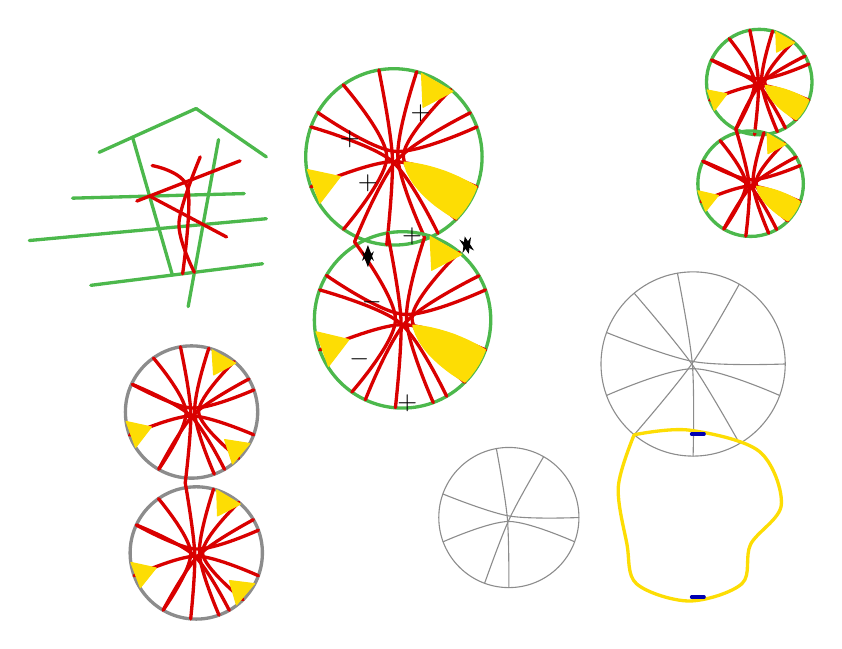
\begin{tikzpicture}[x=1mm,y=1mm,line cap=round,line join=round,font=\scriptsize]
\draw[Lg,very thick] (0.6,-27.92) -- (30.7,-25.15);
\draw[Lg,very thick] (8.41,-33.61) -- (30.22,-30.87);
\draw[Lg,very thick] (6.09,-22.54) -- (27.89,-21.96);
\draw[Lg,very thick] (9.46,-16.72) -- (21.78,-11.16);
\draw[Lg,very thick] (21.78,-11.16) -- (30.7,-17.3);
\draw[Lg,very thick] (13.71,-14.8) -- (18.77,-32.31);
\draw[Lg,very thick] (24.63,-15.1) -- (20.77,-36.31);
\draw[Rd,very thick] plot[smooth, tension=0.55] coordinates {(16.2,-18.4) (20.7,-21.2) (20.07,-32.15)};
\draw[Rd,very thick] plot[smooth, tension=0.55] coordinates {(22.3,-17.3) (19.6,-25.7) (21.56,-31.96)};
\draw[Rd,very thick] (14.25,-22.91) -- (27.36,-17.8);
\draw[Rd,very thick] (15.87,-22.28) -- (25.65,-27.47);
\draw[Lg,very thick] (46.9,-17.3) circle[radius=11.2];
\draw[Rd,very thick] plot[smooth, tension=0.55] coordinates {(44.99,-6.26) (46.7,-17.3) (45.99,-28.46)};
\draw[Rd,very thick] plot[smooth, tension=0.55] coordinates {(49.8,-6.48) (47.4,-17.3) (50.8,-27.5)};
\draw[Rd,very thick] plot[smooth, tension=0.55] coordinates {(40.46,-8.14) (46,-17.3) (40.5,-26.49)};
\draw[Rd,very thick] plot[smooth, tension=0.55] coordinates {(54.14,-8.75) (48.1,-17.3) (54.82,-25.22)};
\draw[Rd,very thick] plot[smooth, tension=0.55] coordinates {(37.23,-11.66) (47,-16.6) (57.43,-13.49)};
\draw[Rd,very thick] plot[smooth, tension=0.55] coordinates {(36.37,-21.11) (46.9,-17.9) (57.43,-21.11)};
\draw[Rd,very thick] plot[smooth, tension=0.55] coordinates {(56.6,-11.7) (47.3,-17.7) (41.9,-28.1)};
\draw[Rd,very thick] plot[smooth, tension=0.55] coordinates {(36.37,-13.49) (46.6,-17.8) (52.5,-27)};
\draw[Ye] (54.4,-9) -- (50.4,-6.7) -- (50.6,-11) -- cycle;
\fill[pattern=north east lines,Ye] (54.4,-9) -- (50.4,-6.7) -- (50.6,-11) -- cycle;
\draw[Ye] (35.9,-18.9) -- (37.5,-23.2) -- (40.1,-19.8) -- cycle;
\fill[pattern=north east lines,Ye] (35.9,-18.9) -- (37.5,-23.2) -- (40.1,-19.8) -- cycle;
\draw[Ye] (54.82,-25.22) -- (55.48,-24.5) -- (56.07,-23.72) -- (56.6,-22.9) -- (57.05,-22.03) -- (57.42,-21.13) -- (57.43,-21.11) -- (57.36,-21.06) -- (57.15,-20.93) -- (56.81,-20.73) -- (56.36,-20.47) -- (55.79,-20.18) -- (55.11,-19.85) -- (54.34,-19.51) -- (53.48,-19.16) -- (52.54,-18.84) -- (51.52,-18.54) -- (50.44,-18.28) -- (49.31,-18.08) -- (48.19,-17.95) -- (48.23,-18.25) -- (48.53,-19.16) -- (48.97,-20.03) -- (49.51,-20.85) -- (50.14,-21.61) -- (50.82,-22.32) -- (51.53,-22.96) -- (52.23,-23.53) -- (52.91,-24.02) -- (53.52,-24.44) -- (54.05,-24.77) -- (54.46,-25.02) -- (54.72,-25.17) -- cycle;
\fill[pattern=north east lines,Ye] (54.82,-25.22) -- (55.48,-24.5) -- (56.07,-23.72) -- (56.6,-22.9) -- (57.05,-22.03) -- (57.42,-21.13) -- (57.43,-21.11) -- (57.36,-21.06) -- (57.15,-20.93) -- (56.81,-20.73) -- (56.36,-20.47) -- (55.79,-20.18) -- (55.11,-19.85) -- (54.34,-19.51) -- (53.48,-19.16) -- (52.54,-18.84) -- (51.52,-18.54) -- (50.44,-18.28) -- (49.31,-18.08) -- (48.19,-17.95) -- (48.23,-18.25) -- (48.53,-19.16) -- (48.97,-20.03) -- (49.51,-20.85) -- (50.14,-21.61) -- (50.82,-22.32) -- (51.53,-22.96) -- (52.23,-23.53) -- (52.91,-24.02) -- (53.52,-24.44) -- (54.05,-24.77) -- (54.46,-25.02) -- (54.72,-25.17) -- cycle;
\draw[Lg,very thick] (48,-38) circle[radius=11.2];
\draw[Rd,very thick] plot[smooth, tension=0.55] coordinates {(46.09,-26.96) (47.8,-38) (47.09,-49.16)};
\draw[Rd,very thick] plot[smooth, tension=0.55] coordinates {(50.8,-27.5) (48.5,-38) (51.9,-48.5)};
\draw[Rd,very thick] plot[smooth, tension=0.55] coordinates {(41.9,-28.1) (47.1,-38) (41.56,-47.16)};
\draw[Rd,very thick] plot[smooth, tension=0.55] coordinates {(55.19,-29.41) (49.2,-37.9) (55.92,-45.92)};
\draw[Rd,very thick] plot[smooth, tension=0.55] coordinates {(38.33,-32.36) (48.1,-37.3) (58.53,-34.19)};
\draw[Rd,very thick] plot[smooth, tension=0.55] coordinates {(37.47,-41.81) (48,-38.6) (58.53,-41.81)};
\draw[Rd,very thick] plot[smooth, tension=0.55] coordinates {(57.7,-32.4) (48.4,-38.3) (43.27,-48.15)};
\draw[Rd,very thick] plot[smooth, tension=0.55] coordinates {(37.47,-34.19) (47.7,-38.4) (53.6,-47.7)};
\draw[Ye] (55.5,-29.7) -- (51.5,-27.4) -- (51.7,-31.7) -- cycle;
\fill[pattern=north east lines,Ye] (55.5,-29.7) -- (51.5,-27.4) -- (51.7,-31.7) -- cycle;
\draw[Ye] (37,-39.5) -- (38.6,-43.9) -- (41.2,-40.5) -- cycle;
\fill[pattern=north east lines,Ye] (37,-39.5) -- (38.6,-43.9) -- (41.2,-40.5) -- cycle;
\draw[Ye] (55.92,-45.92) -- (56.58,-45.2) -- (57.17,-44.42) -- (57.7,-43.6) -- (58.15,-42.73) -- (58.52,-41.83) -- (58.53,-41.81) -- (58.46,-41.76) -- (58.25,-41.63) -- (57.91,-41.43) -- (57.46,-41.17) -- (56.89,-40.88) -- (56.21,-40.55) -- (55.44,-40.21) -- (54.58,-39.86) -- (53.64,-39.54) -- (52.62,-39.24) -- (51.54,-38.98) -- (50.41,-38.78) -- (49.31,-38.66) -- (49.34,-38.86) -- (49.64,-39.77) -- (50.07,-40.65) -- (50.62,-41.48) -- (51.25,-42.25) -- (51.93,-42.96) -- (52.64,-43.61) -- (53.34,-44.19) -- (54.01,-44.7) -- (54.62,-45.12) -- (55.15,-45.46) -- (55.56,-45.71) -- (55.82,-45.87) -- cycle;
\fill[pattern=north east lines,Ye] (55.92,-45.92) -- (56.58,-45.2) -- (57.17,-44.42) -- (57.7,-43.6) -- (58.15,-42.73) -- (58.52,-41.83) -- (58.53,-41.81) -- (58.46,-41.76) -- (58.25,-41.63) -- (57.91,-41.43) -- (57.46,-41.17) -- (56.89,-40.88) -- (56.21,-40.55) -- (55.44,-40.21) -- (54.58,-39.86) -- (53.64,-39.54) -- (52.62,-39.24) -- (51.54,-38.98) -- (50.41,-38.78) -- (49.31,-38.66) -- (49.34,-38.86) -- (49.64,-39.77) -- (50.07,-40.65) -- (50.62,-41.48) -- (51.25,-42.25) -- (51.93,-42.96) -- (52.64,-43.61) -- (53.34,-44.19) -- (54.01,-44.7) -- (54.62,-45.12) -- (55.15,-45.46) -- (55.56,-45.71) -- (55.82,-45.87) -- cycle;
\node[inner sep=1pt] at (50.3,-11.7) {\small $+$};
\node[inner sep=1pt] at (41.3,-15.1) {\small $+$};
\node[inner sep=1pt] at (43.6,-20.7) {\small $+$};
\node[inner sep=1pt] at (49.2,-27.4) {\small $+$};
\node[inner sep=1pt] at (48.6,-48.6) {\small $+$};
\node[inner sep=1pt] at (44.1,-35.8) {\small $-$};
\node[inner sep=1pt] at (42.5,-43) {\small $-$};
\draw[{Stealth[length=2mm]}-{Stealth[length=2mm]}] (43.6,-28.5) -- (43.6,-31.3);
\draw[{Stealth[length=2mm]}-{Stealth[length=2mm]}] (55.9,-27.4) -- (56.4,-29.6);
\draw[pencil,very thick] (21.2,-49.7) circle[radius=8.4];
\draw[Rd,very thick] plot[smooth, tension=0.55] coordinates {(19.79,-41.42) (21.1,-49.7) (20.4,-58.7)};
\draw[Rd,very thick] plot[smooth, tension=0.55] coordinates {(23.4,-41.59) (21.6,-49.7) (24.09,-57.59)};
\draw[Rd,very thick] plot[smooth, tension=0.55] coordinates {(16.36,-42.84) (20.5,-49.7) (17.05,-56.95)};
\draw[Rd,very thick] plot[smooth, tension=0.55] coordinates {(26.62,-43.28) (22.1,-49.7) (27.19,-55.59)};
\draw[Rd,very thick] plot[smooth, tension=0.55] coordinates {(13.7,-46.2) (21.3,-49.2) (29.12,-46.89)};
\draw[Rd,very thick] plot[smooth, tension=0.55] coordinates {(13.33,-52.63) (21.2,-50.2) (29.09,-52.59)};
\draw[Rd,very thick] plot[smooth, tension=0.55] coordinates {(28.48,-45.51) (21.5,-50) (17.05,-56.95)};
\draw[Rd,very thick] plot[smooth, tension=0.55] coordinates {(13.7,-46.2) (21,-50.1) (25.39,-56.98)};
\draw[Ye] (26.8,-43.5) -- (23.8,-41.8) -- (24,-45) -- cycle;
\fill[pattern=north east lines,Ye] (26.8,-43.5) -- (23.8,-41.8) -- (24,-45) -- cycle;
\draw[Ye] (12.9,-50.9) -- (14.1,-54.2) -- (16.1,-51.6) -- cycle;
\fill[pattern=north east lines,Ye] (12.9,-50.9) -- (14.1,-54.2) -- (16.1,-51.6) -- cycle;
\draw[Ye] (26.4,-56.3) -- (28.6,-53.7) -- (25.4,-53.2) -- cycle;
\fill[pattern=north east lines,Ye] (26.4,-56.3) -- (28.6,-53.7) -- (25.4,-53.2) -- cycle;
\draw[pencil,very thick] (21.8,-67.6) circle[radius=8.4];
\draw[Rd,very thick] plot[smooth, tension=0.55] coordinates {(20.4,-58.7) (21.6,-67.6) (21.09,-75.97)};
\draw[Rd,very thick] plot[smooth, tension=0.55] coordinates {(24,-59.49) (22.2,-67.6) (24.69,-75.49)};
\draw[Rd,very thick] plot[smooth, tension=0.55] coordinates {(17,-60.7) (21.1,-67.6) (17.6,-74.85)};
\draw[Rd,very thick] plot[smooth, tension=0.55] coordinates {(27.22,-61.18) (22.6,-67.6) (27.74,-73.54)};
\draw[Rd,very thick] plot[smooth, tension=0.55] coordinates {(14.2,-64.05) (21.8,-67.1) (29.69,-64.71)};
\draw[Rd,very thick] plot[smooth, tension=0.55] coordinates {(13.91,-70.49) (21.8,-68) (29.69,-70.49)};
\draw[Rd,very thick] plot[smooth, tension=0.55] coordinates {(29.06,-63.37) (22.1,-67.9) (17.6,-74.85)};
\draw[Rd,very thick] plot[smooth, tension=0.55] coordinates {(14.2,-64.05) (21.5,-67.9) (25.99,-74.88)};
\draw[Ye] (27.4,-61.4) -- (24.4,-59.6) -- (24.5,-62.9) -- cycle;
\fill[pattern=north east lines,Ye] (27.4,-61.4) -- (24.4,-59.6) -- (24.5,-62.9) -- cycle;
\draw[Ye] (13.5,-68.8) -- (14.7,-72) -- (16.7,-69.5) -- cycle;
\fill[pattern=north east lines,Ye] (13.5,-68.8) -- (14.7,-72) -- (16.7,-69.5) -- cycle;
\draw[Ye] (26.9,-74.2) -- (29.2,-71.5) -- (26,-71.1) -- cycle;
\fill[pattern=north east lines,Ye] (26.9,-74.2) -- (29.2,-71.5) -- (26,-71.1) -- cycle;
\draw[Lg,very thick] (93.3,-7.8) circle[radius=6.7];
\draw[Rd,very thick] plot[smooth, tension=0.55] coordinates {(92.1,-1.21) (93.2,-7.8) (92.7,-14.47)};
\draw[Rd,very thick] plot[smooth, tension=0.55] coordinates {(95,-1.32) (93.6,-7.8) (95.6,-14.09)};
\draw[Rd,very thick] plot[smooth, tension=0.55] coordinates {(89.49,-2.29) (92.7,-7.8) (90.33,-13.77)};
\draw[Rd,very thick] plot[smooth, tension=0.55] coordinates {(97.62,-2.68) (94,-7.8) (97.99,-12.59)};
\draw[Rd,very thick] plot[smooth, tension=0.55] coordinates {(87.25,-5) (93.3,-7.4) (99.59,-5.5)};
\draw[Rd,very thick] plot[smooth, tension=0.55] coordinates {(87.01,-10.1) (93.3,-8.2) (99.59,-10.1)};
\draw[Rd,very thick] plot[smooth, tension=0.55] coordinates {(99.12,-4.49) (93.5,-8) (90.33,-13.77)};
\draw[Rd,very thick] plot[smooth, tension=0.55] coordinates {(87.25,-5) (93.1,-8.1) (96.61,-13.62)};
\draw[Ye] (97.8,-2.8) -- (95.4,-1.4) -- (95.5,-4) -- cycle;
\fill[pattern=north east lines,Ye] (97.8,-2.8) -- (95.4,-1.4) -- (95.5,-4) -- cycle;
\draw[Ye] (86.7,-8.8) -- (87.6,-11.4) -- (89.2,-9.3) -- cycle;
\fill[pattern=north east lines,Ye] (86.7,-8.8) -- (87.6,-11.4) -- (89.2,-9.3) -- cycle;
\draw[Ye] (97.98,-12.59) -- (98.04,-12.54) -- (98.43,-12.11) -- (98.79,-11.64) -- (99.1,-11.15) -- (99.37,-10.63) -- (99.59,-10.1) -- (99.55,-10.07) -- (99.43,-9.99) -- (99.23,-9.87) -- (98.95,-9.72) -- (98.61,-9.54) -- (98.21,-9.35) -- (97.74,-9.15) -- (97.23,-8.95) -- (96.67,-8.75) -- (96.06,-8.58) -- (95.42,-8.42) -- (94.74,-8.31) -- (94.06,-8.23) -- (94.08,-8.37) -- (94.25,-8.92) -- (94.51,-9.45) -- (94.83,-9.94) -- (95.21,-10.4) -- (95.61,-10.83) -- (96.03,-11.22) -- (96.45,-11.56) -- (96.85,-11.86) -- (97.21,-12.11) -- (97.53,-12.32) -- (97.77,-12.47) -- (97.93,-12.56) -- cycle;
\fill[pattern=north east lines,Ye] (97.98,-12.59) -- (98.04,-12.54) -- (98.43,-12.11) -- (98.79,-11.64) -- (99.1,-11.15) -- (99.37,-10.63) -- (99.59,-10.1) -- (99.55,-10.07) -- (99.43,-9.99) -- (99.23,-9.87) -- (98.95,-9.72) -- (98.61,-9.54) -- (98.21,-9.35) -- (97.74,-9.15) -- (97.23,-8.95) -- (96.67,-8.75) -- (96.06,-8.58) -- (95.42,-8.42) -- (94.74,-8.31) -- (94.06,-8.23) -- (94.08,-8.37) -- (94.25,-8.92) -- (94.51,-9.45) -- (94.83,-9.94) -- (95.21,-10.4) -- (95.61,-10.83) -- (96.03,-11.22) -- (96.45,-11.56) -- (96.85,-11.86) -- (97.21,-12.11) -- (97.53,-12.32) -- (97.77,-12.47) -- (97.93,-12.56) -- cycle;
\draw[Lg,very thick] (92.2,-20.7) circle[radius=6.7];
\draw[Rd,very thick] plot[smooth, tension=0.55] coordinates {(90.33,-13.77) (92,-20.7) (91.59,-27.37)};
\draw[Rd,very thick] plot[smooth, tension=0.55] coordinates {(93.9,-14.22) (92.5,-20.7) (94.5,-26.99)};
\draw[Rd,very thick] plot[smooth, tension=0.55] coordinates {(88.32,-15.23) (91.6,-20.7) (88.8,-26.45)};
\draw[Rd,very thick] plot[smooth, tension=0.55] coordinates {(96.47,-15.54) (92.9,-20.6) (96.94,-25.44)};
\draw[Rd,very thick] plot[smooth, tension=0.55] coordinates {(86.15,-17.85) (92.2,-20.2) (98.49,-18.4)};
\draw[Rd,very thick] plot[smooth, tension=0.55] coordinates {(85.91,-23) (92.2,-21) (98.49,-23)};
\draw[Rd,very thick] plot[smooth, tension=0.55] coordinates {(97.98,-17.31) (92.4,-20.9) (88.8,-26.45)};
\draw[Rd,very thick] plot[smooth, tension=0.55] coordinates {(86.15,-17.85) (92,-20.9) (95.51,-26.52)};
\draw[Ye] (96.7,-15.7) -- (94.3,-14.3) -- (94.4,-16.9) -- cycle;
\fill[pattern=north east lines,Ye] (96.7,-15.7) -- (94.3,-14.3) -- (94.4,-16.9) -- cycle;
\draw[Ye] (85.5,-21.6) -- (86.5,-24.2) -- (88.1,-22.2) -- cycle;
\fill[pattern=north east lines,Ye] (85.5,-21.6) -- (86.5,-24.2) -- (88.1,-22.2) -- cycle;
\draw[Ye] (96.94,-25.44) -- (97.33,-25.01) -- (97.69,-24.54) -- (98,-24.05) -- (98.27,-23.53) -- (98.49,-23) -- (98.45,-22.97) -- (98.33,-22.89) -- (98.13,-22.76) -- (97.85,-22.6) -- (97.51,-22.42) -- (97.11,-22.21) -- (96.64,-22) -- (96.13,-21.79) -- (95.57,-21.58) -- (94.96,-21.4) -- (94.32,-21.24) -- (93.64,-21.11) -- (92.96,-21.03) -- (92.98,-21.17) -- (93.16,-21.73) -- (93.43,-22.25) -- (93.76,-22.75) -- (94.13,-23.22) -- (94.54,-23.65) -- (94.97,-24.04) -- (95.39,-24.39) -- (95.79,-24.7) -- (96.16,-24.95) -- (96.47,-25.16) -- (96.72,-25.31) -- (96.88,-25.41) -- cycle;
\fill[pattern=north east lines,Ye] (96.94,-25.44) -- (97.33,-25.01) -- (97.69,-24.54) -- (98,-24.05) -- (98.27,-23.53) -- (98.49,-23) -- (98.45,-22.97) -- (98.33,-22.89) -- (98.13,-22.76) -- (97.85,-22.6) -- (97.51,-22.42) -- (97.11,-22.21) -- (96.64,-22) -- (96.13,-21.79) -- (95.57,-21.58) -- (94.96,-21.4) -- (94.32,-21.24) -- (93.64,-21.11) -- (92.96,-21.03) -- (92.98,-21.17) -- (93.16,-21.73) -- (93.43,-22.25) -- (93.76,-22.75) -- (94.13,-23.22) -- (94.54,-23.65) -- (94.97,-24.04) -- (95.39,-24.39) -- (95.79,-24.7) -- (96.16,-24.95) -- (96.47,-25.16) -- (96.72,-25.31) -- (96.88,-25.41) -- cycle;
\draw[pencil] (61.5,-63.1) circle[radius=8.9];
\draw[pencil] plot[smooth, tension=0.55] coordinates {(59.91,-54.34) (61.3,-63.1) (61.5,-72)};
\draw[pencil] plot[smooth, tension=0.55] coordinates {(65.92,-55.37) (61.6,-63.2) (58.42,-71.45)};
\draw[pencil] plot[smooth, tension=0.55] coordinates {(53.12,-60.11) (61.5,-62.9) (70.4,-63.1)};
\draw[pencil] plot[smooth, tension=0.55] coordinates {(53.15,-66.18) (61.5,-63.6) (69.85,-66.18)};
\draw[pencil] (84.9,-43.6) circle[radius=11.7];
\draw[pencil] plot[smooth, tension=0.55] coordinates {(82.91,-32.07) (84.8,-43.6) (84.9,-55.3)};
\draw[pencil] plot[smooth, tension=0.55] coordinates {(90.76,-33.47) (84.8,-43.5) (77.41,-52.59)};
\draw[pencil] plot[smooth, tension=0.55] coordinates {(73.9,-39.6) (85,-43.3) (96.6,-43.6)};
\draw[pencil] plot[smooth, tension=0.55] coordinates {(73.9,-47.6) (84.9,-44.2) (95.9,-47.6)};
\draw[pencil] plot[smooth, tension=0.55] coordinates {(77.41,-34.61) (84.8,-43.7) (90.8,-53.7)};
\draw[Ye,very thick] plot[smooth, tension=0.55] coordinates {(77.41,-52.59) (84.4,-52) (93.3,-54.7) (96.1,-61.5) (92.2,-66.5) (91.1,-71.5) (84.4,-73.7) (77.7,-71.5) (76.5,-66.5) (75.4,-59.2) (77.41,-52.59)};
\draw[Bl,very thick] (84.7,-52.5) -- (86.3,-52.5);
\draw[Bl,very thick] (84.7,-73.2) -- (86.3,-73.2);
\end{tikzpicture}
\end{document}
